% Options for packages loaded elsewhere
\PassOptionsToPackage{unicode}{hyperref}
\PassOptionsToPackage{hyphens}{url}
%
\documentclass[
]{article}
\usepackage{amsmath,amssymb}
\usepackage{lmodern}
\usepackage{iftex}
\ifPDFTeX
  \usepackage[T1]{fontenc}
  \usepackage[utf8]{inputenc}
  \usepackage{textcomp} % provide euro and other symbols
\else % if luatex or xetex
  \usepackage{unicode-math}
  \defaultfontfeatures{Scale=MatchLowercase}
  \defaultfontfeatures[\rmfamily]{Ligatures=TeX,Scale=1}
\fi
% Use upquote if available, for straight quotes in verbatim environments
\IfFileExists{upquote.sty}{\usepackage{upquote}}{}
\IfFileExists{microtype.sty}{% use microtype if available
  \usepackage[]{microtype}
  \UseMicrotypeSet[protrusion]{basicmath} % disable protrusion for tt fonts
}{}
\usepackage{xcolor}
\IfFileExists{xurl.sty}{\usepackage{xurl}}{} % add URL line breaks if available
\IfFileExists{bookmark.sty}{\usepackage{bookmark}}{\usepackage{hyperref}}
\hypersetup{
  pdftitle={CI mispronunciation sensitivity: results},
  pdfauthor={Meg Cychosz},
  hidelinks,
  pdfcreator={LaTeX via pandoc}}
\urlstyle{same} % disable monospaced font for URLs
\usepackage[margin=1in]{geometry}
\usepackage{longtable,booktabs,array}
\usepackage{calc} % for calculating minipage widths
% Correct order of tables after \paragraph or \subparagraph
\usepackage{etoolbox}
\makeatletter
\patchcmd\longtable{\par}{\if@noskipsec\mbox{}\fi\par}{}{}
\makeatother
% Allow footnotes in longtable head/foot
\IfFileExists{footnotehyper.sty}{\usepackage{footnotehyper}}{\usepackage{footnote}}
\makesavenoteenv{longtable}
\usepackage{graphicx}
\makeatletter
\def\maxwidth{\ifdim\Gin@nat@width>\linewidth\linewidth\else\Gin@nat@width\fi}
\def\maxheight{\ifdim\Gin@nat@height>\textheight\textheight\else\Gin@nat@height\fi}
\makeatother
% Scale images if necessary, so that they will not overflow the page
% margins by default, and it is still possible to overwrite the defaults
% using explicit options in \includegraphics[width, height, ...]{}
\setkeys{Gin}{width=\maxwidth,height=\maxheight,keepaspectratio}
% Set default figure placement to htbp
\makeatletter
\def\fps@figure{htbp}
\makeatother
\setlength{\emergencystretch}{3em} % prevent overfull lines
\providecommand{\tightlist}{%
  \setlength{\itemsep}{0pt}\setlength{\parskip}{0pt}}
\setcounter{secnumdepth}{5}
\usepackage{booktabs}
\usepackage{longtable}
\usepackage{array}
\usepackage{multirow}
\usepackage{wrapfig}
\usepackage{float}
\usepackage{colortbl}
\usepackage{pdflscape}
\usepackage{tabu}
\usepackage{threeparttable}
\usepackage{threeparttablex}
\usepackage[normalem]{ulem}
\usepackage{makecell}
\ifLuaTeX
  \usepackage{selnolig}  % disable illegal ligatures
\fi

\title{CI mispronunciation sensitivity: results}
\author{Meg Cychosz}
\date{17 May 2022}

\begin{document}
\maketitle

\begin{table}[!h]

\caption{\label{tab:demo-tab}Participant demographic information (N=19 matches), Mean (SD), range.}
\centering
\begin{tabular}[t]{lllllll}
\toprule
Hearing Status & Girls, Boys & Chronological Age: months & Hearing Age: months & Maternal Education Level & EVT-2 GSV Scores & EVT-2 Stan. Scores\\
\midrule
CochlearImplant & 13 , 6 & 56.32 ( 6.71 ) 44 - 66 & 44.47 ( 8.69 ) 29 - 56 & 6.26 ( 0.56 ) & 134.84 ( 12 ) 112 - 159 & 102.63 ( 13.37 ) 84 - 131\\
NormalHearing & 13 , 6 & 45.47 ( 7.46 ) 36 - 57 & 45.47 ( 7.46 ) 36 - 57 & 6.05 ( 0.62 ) & 132.68 ( 10.88 ) 117 - 150 & 114.58 ( 10.38 ) 98 - 134\\
\bottomrule
\end{tabular}
\end{table}

\hypertarget{results}{%
\section{Results}\label{results}}

\hypertarget{analysis-plan}{%
\subsection{Analysis plan}\label{analysis-plan}}

We evaluate the mispronunciation sensitivity of children with CIs in comparison to their hearing age- and vocabulary size-matched peers. The outcome variable is the proportion of looks to the familiar object versus the unfamiliar object, over time (300--1,800 ms after target word onset), which we modeled using Generalized Additive Mixed Models (GAMMs). GAMMs have become an important tool to model time series data, such as eyetracking trajectories, because they can incorporate nonlinear relationships between variables such as time, response, and relevant covariates (i.e., effects of group and/or condition) (rijChildrenEyeGaze2016;zahnerAlignmentF0Peak). GAMMs are composed of (fixed) \emph{parametric} terms that model static relationships between two variables, as is common in generalized linear modeling, and \emph{smooth} terms that model nonlinear effects by using penalized basis functions (smoothing splines). Parametric terms can be interpreted from model summaries, as in traditional regression, but smooth terms must be interpreted visually. Wieling (2017) and Sóskuthy (2021) provide tutorials for GAMMs in language research and Wood (2017) provides a comprehensive textbook treatment of the approach.

GAMMs also allow for autocorrelation between observations to be factored into the modeling. Incorporating autocorrelation is of particular importance to eyetracking data where we anticipate large amounts of within-trial correlation between measurements over time: the area where the child is looking at 500ms is highly correlated with where they are looking at 550ms. As such, GAMMs are a significant improvement upon other polynomial regression models common in time series analysis, such as Growth Curve Models (GCMs). The standard approach for estimating GCMs cannot factor in this inherent correlational structure within the data and, as a result, recent work has shown that they result in inflated Type I error rates (Huang \& Snedeker, 2020).

The current data were analyzed in the RStudio computing environment (R version 4.0.2; Rcite). All computing and statistical analyses are included in the GitHub repository affiliated with this project \textless github.com/megseekosh/ci-mispron\textgreater. Visualizations were made using the ggplot2 and cowplot packages. Modeling was conducted and presented using the mgcv, itsadug, and tidymv packages. For all modeling, the proportion of children's looks to the familiar object versus the unfamiliar object was calculated for each frame (every 50 ms) and transformed to empirical logit (elog), or the log-odds of looking to the familiar object at each sample (Barr, 2008). Random effects (``factor smooths'' in GAMMs) included by-participant, by-observation (first {[}at age 3{]}, second {[}at age 4{]}, or third {[}at age 5{]} visit to the lab), and by-item trajectories. These factor smooths modeled variability stemming from individual children and lexical items, and took into account the repeated observations from some children at two different ages. To ensure assumptions were met and to avoid overfitting, model criticism was conducted using the gam.check() function; when necessary, the basis function number (\emph{k} or knots) was increased.

As is common in eye-tracking data, the response data were distributed with heavy tails. Consequently, all models were fit using a scaled-t model using the ``scat'' link function, which substantially improved data distribution (woodSmoothingParameterModel2016). Finally, for each model, autocorrelation between model residuals was calculated; all models showed high amounts of autocorrelation. These dependencies were factored into the modeling by fitting an autoregressive error model (AR(1)) that modeled the degree of autocorrelation (\emph{rho}) between timepoints in each trial. Subsequent model inspection demonstrated that specifying this autocorrelation value in the model sufficiently factored out autocorrelation between residuals (Wieling, 2017).

\hypertarget{evaluating-the-effect-of-phonetic-detail-on-mispronunciation-sensitivity}{%
\subsection{Evaluating the effect of phonetic detail on mispronunciation sensitivity}\label{evaluating-the-effect-of-phonetic-detail-on-mispronunciation-sensitivity}}

To evaluate how access to fine, phonetic detail may affect mispronunciation sensitivity, a series of GAMMs were fit comparing children with CIs and their hearing age- and vocabulary size-matched TH peers. \textbf{Condition} (Correct Pronunciation vs.~Mispronunciation) was contrast-coded to facilitate model interpretation and the 2x2 relationship of \textbf{Group} (Children with CIs vs.~TH) and \textbf{Condition} was modeled using ordered factors. A model with parametric and smooth terms for \textbf{Group} and \textbf{Condition} improved upon a \textbf{Condition}-only model, suggesting that children with CIs and TH responded differently to correct- versus mis-pronunciations.

To statistically evaluate the source of the \textbf{Group} effect (i.e., stemming from overall vs.~time-varying response to the stimuli), another model was fit that included parametric terms for \textbf{Group}, and the ordered factors of \emph{Correct Pronunciation} for children with CIs and \emph{Correct Pronunciation} for children with TH (Wieling, 2017). These parametric effects modeled the constant effect (the intercept) of the covariates upon the response variable. Smooth model terms included non-linear effects of \textbf{Time} and \textbf{Time} by \textbf{Group}. The latter allowed us to model the non-linear difference between the two different groups' responses to mispronunciations. Finally, the model included difference smooths, which allowed us to separately model how each hearing group responded to correct- versus mis-pronunciations, over time. See Table \ref{tab:2-by-2-model-summary} for model summary.

\begin{verbatim}
## % latex table generated in R 4.0.2 by xtable 1.8-4 package
## % Tue May 17 12:23:51 2022
## \begin{table}[ht]
## \centering
## \begin{tabular}{lrrrr}
##    \hline
## A. parametric coefficients & Estimate & Std. Error & t-value & p-value \\ 
##   Intercept (Cochlear Implant: Mispronunciation) & 0.2662 & 0.1920 & 1.3868 & 0.1655 \\ 
##   Typical Hearing & -0.3259 & 0.1924 & -1.6932 & 0.0904 \\ 
##   Typical Hearing: Correct & 1.1826 & 0.2259 & 5.2363 & $<$ 0.0001 \\ 
##   Cochlear Implant: Correct & 0.6789 & 0.2252 & 3.0138 & 0.0026 \\ 
##    \hline
## B. smooth terms & edf & Ref.df & F-value & p-value \\ 
##   s(Time) & 0.0002 & 0.0004 & 755.4057 & 0.5803 \\ 
##   s(Time,Cochlear Implant) & 1.0001 & 1.0002 & 2.6265 & 0.1055 \\ 
##   s(Time,Typical Hearing) & 3.2556 & 4.1432 & 1.3554 & 0.2429 \\ 
##   s(Time,Typical Hearing; Correct) & 5.0601 & 6.3159 & 8.6538 & $<$ 0.0001 \\ 
##   s(Time,Cochlear Implant; Correct) & 3.7598 & 4.8315 & 7.2809 & $<$ 0.0001 \\ 
##   s(Time,Child) & 52.1753 & 341.0000 & 0.4680 & $<$ 0.0001 \\ 
##   s(Time,Item) & 25.5375 & 108.0000 & 0.6854 & $<$ 0.0001 \\ 
##   s(Time,Observation) & 0.0010 & 27.0000 & 0.1394 & $<$ 0.0001 \\ 
##    \hline
## \end{tabular}
## \caption{Model summary predicting the difference between proportion of looks to the familiar object by word condition and hearing status.} 
## \label{2-by-2-model-summary}
## \end{table}
\end{verbatim}

In the first part of the results, we ask: are both children with CIs and their TH matches sensitive to mispronunciations? Parametric effects in the model summary show that there are, overall, significantly more looks to the familiar photo for \emph{Correct Pronunciation} trials than \emph{Mispronunciation} trials, for both children with CIs and TH (CI logit Est.=0.68, p\textless.001, or proportion Est: 0.2106274; TH logit Est.=1.18, p\textless.001, or proportion Est: 0.30632). we interpret the smooth terms by first considering effective degrees of freedom (EDF) and the significance test for each smooth. The EDF indicates how much wiggliness there is in a smooth where EDF=1 indicates a linear relationship and a larger value indicates more wiggliness in the smooth. Interpretation of the non-linear smooths shows that there are significant, non-linear differences in looks to the familiar object between correct- and mis-pronunciations for children with CIs (smooth of \textbf{Time} by the ordered \textbf{Cochlear Implant; Correct}) and children with TH (smooth of \textbf{Time} by the ordered \textbf{Typical Hearing; Correct}) (Figure \ref{fig:2x2-plot}). Thus, both children with CIs and TH are sensitive to mispronunciations.

\begin{figure}
\centering
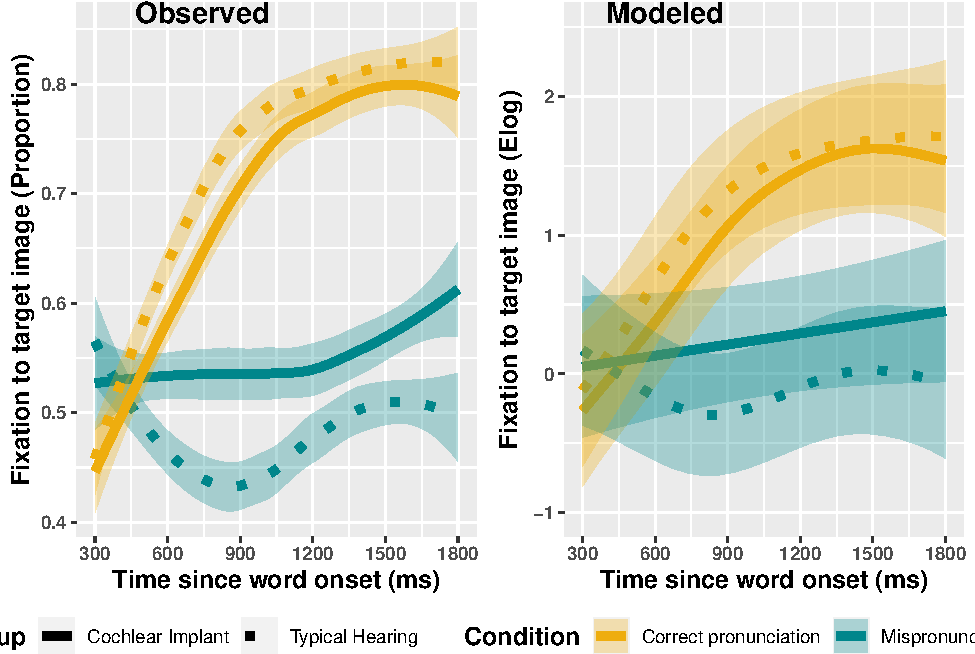
\includegraphics{2_modeling_files/figure-latex/2x2-plot-1.pdf}
\caption{\label{fig:2x2-plot}Observed data and GAMM predictions for proportion of looks to familiar object, by word condition and hearing status. Fixations on the y-axis are plotted as the empirical logit values (elog). Shaded ribbons represent 95\% confidence intervals.}
\end{figure}

Nevertheless, the above modeling cannot tell us if these children with CIs are \emph{less} sensitive to mispronunciations than their TH peers; the modeling demonstrates only that both groups show sensitivity. To evaluate differences in mispronunciation sensitivity by group, another GAMM was fit, with a binary difference smooth, which allowed us to evaluate the \emph{difference} between smooths (Correct- vs.~Mis-pronunciations) for children with CIs and TH, over time. Model fit included parametric effects of \textbf{Group}, as well as smooths of \textbf{Time}, \textbf{Time} by \textbf{Group}, \textbf{Time} by \textbf{Condition}, and \textbf{Time} by the ordered variable of \textbf{Group} by \textbf{Condition} (to model the difference between real- and mis-pronunciations for each group). Model results are plotted in Figure \ref{fig:ci-th-facet-plot}; the model summary is included in supplementary materials. Overall, the model-estimated difference smooths show smaller differences between correct- and mis-pronunciations for the children with CIs---and that these differences take longer to manifest during online processing (left panel of Figure \ref{fig:ci-th-facet-plot}). Further inspection of the first model, as plotted in Figure \ref{fig:real-mp-facet-plot}, demonstrates why this is the case. The children with CIs and TH do not respond significantly differently to correct pronunciations: once vocabulary size and hearing age are controlled, both groups of children respond similarly to correctly-pronounced words. Instead, children with CIs---who are listening with a degraded speech signal via electric hearing---are less sensitive to \emph{mis}-pronunciations (Figure \ref{fig:real-mp-facet-plot}), resulting in smaller difference smooths between correct- and mis-pronunciations.

\begin{figure}
\centering
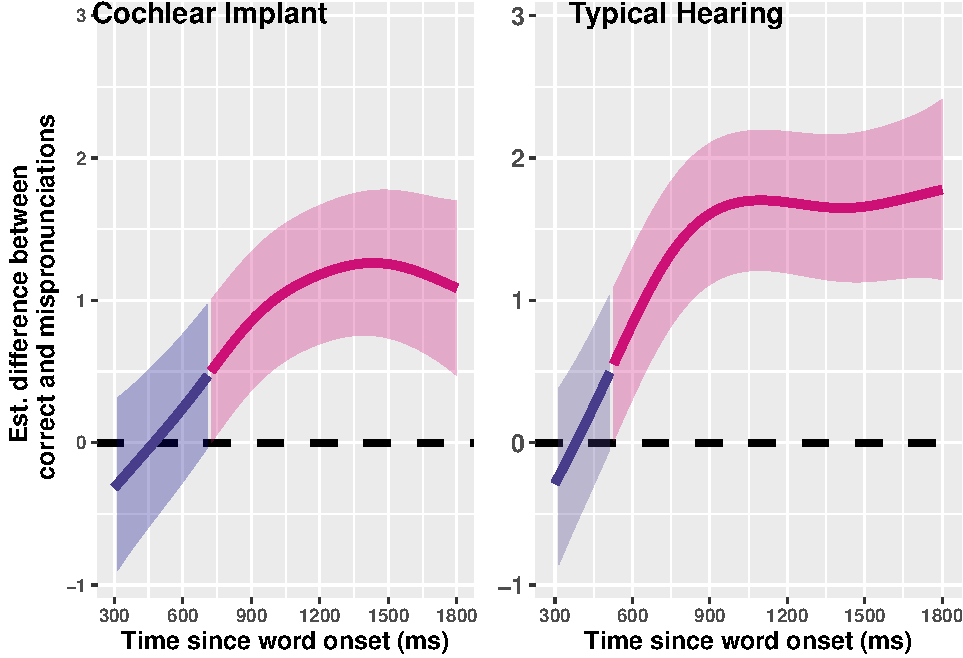
\includegraphics{2_modeling_files/figure-latex/ci-th-facet-plot-1.pdf}
\caption{\label{fig:ci-th-facet-plot}Difference smooths (GAMM predictions) by condition (correct- vs.~mis-pronunciations) for children with CIs (L) and TH (R). Pink smooths represent the point when correct and mis-pronunciation smooths differ (i.e., reliable effect of condition) for each group: there is a larger difference between correct and mispronunciation responses for children with TH than CIs. Shaded ribbons represent 95\% confidence intervals.}
\end{figure}

\begin{figure}
\centering
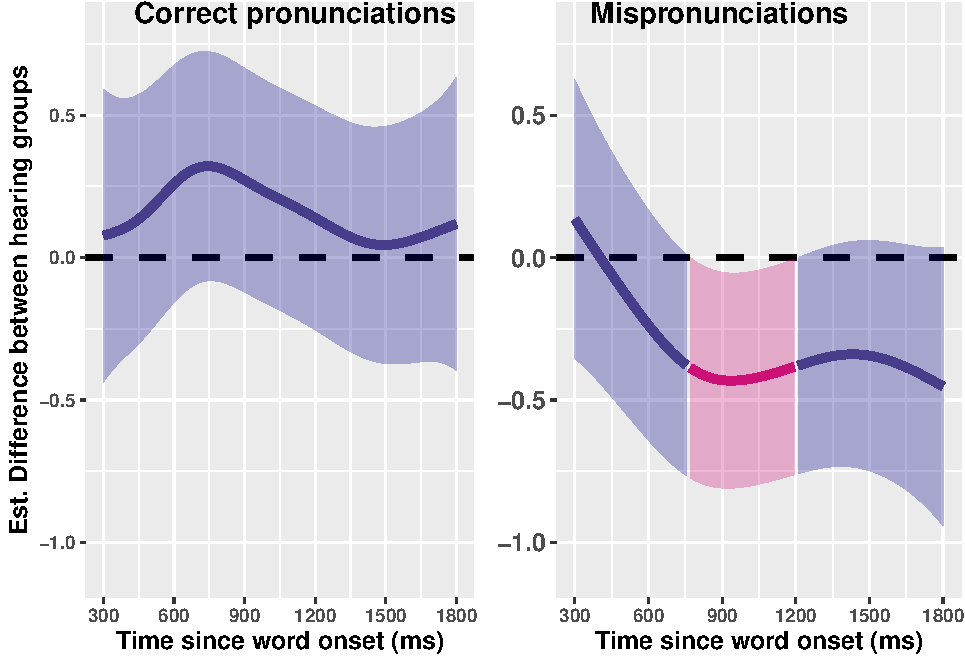
\includegraphics{2_modeling_files/figure-latex/real-mp-facet-plot-1.pdf}
\caption{\label{fig:real-mp-facet-plot}Difference smooths (GAMM predictions) by hearing status for correct pronunciations and mispronunciations. The pink smooth represents the point when the smooth for children with TH differs from children with CIs (i.e., reliable effect of group): there is an effect of group upon mispronunciations (L plot: see also difference between yellow lines in Figure 1), but not correct pronunciations (R plot: see also difference between turquoise lines in Figure 1). Shaded ribbons represent 95\% confidence intervals.}
\end{figure}

\hypertarget{explaining-individual-differences-in-mispronunciation-sensitivity}{%
\subsection{Explaining individual differences in mispronunciation sensitivity}\label{explaining-individual-differences-in-mispronunciation-sensitivity}}

\begin{table}[!h]

\caption{\label{tab:stan-meas-table}Summary statistics of standardized speech-language measures, by hearing status (N=33 children with CIs and N=24 with TH). Mean (SD), range.}
\centering
\begin{tabular}[t]{llll}
\toprule
Hearing Status & EVT-2 standard score & EVT-2 GSVs & GFTA-2 standard score\\
\midrule
CochlearImplant & 95.7 ( 18.71 ) 46 - 127 & 120.76 ( 25.99 ) 42 - 159 & 73.61 ( 19.33 ) 39 - 107\\
NormalHearing & 116.17 ( 12 ) 88 - 134 & 140.46 ( 15.46 ) 117 - 164 & 90.04 ( 12.04 ) 67 - 113\\
\bottomrule
\end{tabular}
\end{table}

\begin{table}[!h]

\caption{\label{tab:demo-tab-allkids}Demographic information of children who completed standardized speech-language measures, by hearing status (N=33 children with CIs and N=24 with TH). Mean (SD), range.}
\centering
\begin{tabular}[t]{lllll}
\toprule
Group & Girls, Boys & Chronological Age: months & Hearing Age: months & Maternal Education Level\\
\midrule
CochlearImplant & 21 , 12 & 50.91 ( 10.01 ) 34 - 66 & 33.33 ( 14.91 ) 5 - 56 & 5.76 ( 1.09 )\\
NormalHearing & 15 , 9 & 52.71 ( 10.81 ) 36 - 66 & 52.71 ( 10.81 ) 36 - 66 & 5.67 ( 1.34 )\\
\bottomrule
\end{tabular}
\end{table}

Having established that children with CIs are less sensitive to mispronunciations than their TH peers, we next correlated the children's responses with two different standardized speech-language assessments: expressive vocabulary size (EVT-2) and spoken phonetic/articulatory accuracy (GFTA-2). Because we took an individual differences approach, we examined the children with CIs and TH separately.

We modeled the effects of vocabulary size and articulation on the children who completed both assessments (N=33 with CIs and N=24 with TH) by using stepwise GAMM fitting. Specifically, we assessed the non-linear interaction between \textbf{Time}, \textbf{Condition}, and \textbf{Vocabulary Score}/\textbf{Phonetic Accuracy} to evaluate if children's vocabulary sizes and/or phonetic accuracy predicted their looks to the target over time for the correct- and mis-pronunciation conditions. As before, all models included factor (random) smooths by participant, observation (visit to the lab), and item. Each additionally included a difference smooth of \textbf{Time} and \textbf{Participant} by \textbf{Condition} (\emph{Correct-} versus \emph{Mis-pronunciation}). A baseline model was fit with a parametric term for \textbf{Condition} (estimating the average looking probability in each condition), smooth terms for \textbf{Time} and \textbf{Time} by \textbf{Condition}, as well as a non-linear interaction (tensor product) of \textbf{Time} and \textbf{Child Age} (modeled continuously) by \textbf{Condition}. In all models we included the Age by Condition tensor product smooth term because our child-level variables (vocabulary score and phonetic accuracy) are confounded with age, and we wanted to evaluate the potential influence of these speech-language abilities independent of child age.

We fit the three-way interaction of \textbf{Time}, \textbf{Condition}, and \textbf{Vocabulary Score} and \textbf{Time}, \textbf{Condition}, and \textbf{Phonetic Accuracy} using tensor product terms. For the children with TH, neither the vocabulary nor phonetic accuracy term improved upon a baseline model controlling for child age. This result indicates that, for the children with TH, mispronunciation sensitivity---the difference in looks to the target image in correct- versus mis-pronunciation conditions---is not moderated by vocabulary size or phonetic accuracy over and above age effects. For the children with CIs, best model fit included \textbf{Phonetic Accuracy}; \textbf{Vocabulary Score} did not improve upon model fit. The final model summary for the children with CIs is included in the supplementary materials.

Given the multiple non-linear effects at play, it is necessary to plot the model predictions in order to interpret GAMM outputs, in particular how phonetic accuracy mediates mispronunciation sensitivity for the children with CIs. To facilitate interpretation of the non-linear three-way interaction, the children with CIs were divided into tertiles by vocabulary score and phonetic accuracy. Predictions from the model, by articulatory tertile, are plotted in Figure \ref{fig:CI-diff-plot} and raw response curves are plotted in Figure \ref{fig:CI-raw-plot}. The model predictions demonstrate that children with better articulation scores show larger differences between looks to the target for correct- versus mis-pronunciations (higher overall \emph{y}-intercept value) and that these children show significant differences between correct- and mis-pronunciations slightly earlier in the analysis window (cross-over from purple to pink smooth occurs sooner in the analysis window). Thus, for the children with CIs, phonetic/articulatory accuracy predicts mispronunciation sensitivity, independent of age and language ability.

\begin{figure}
\centering
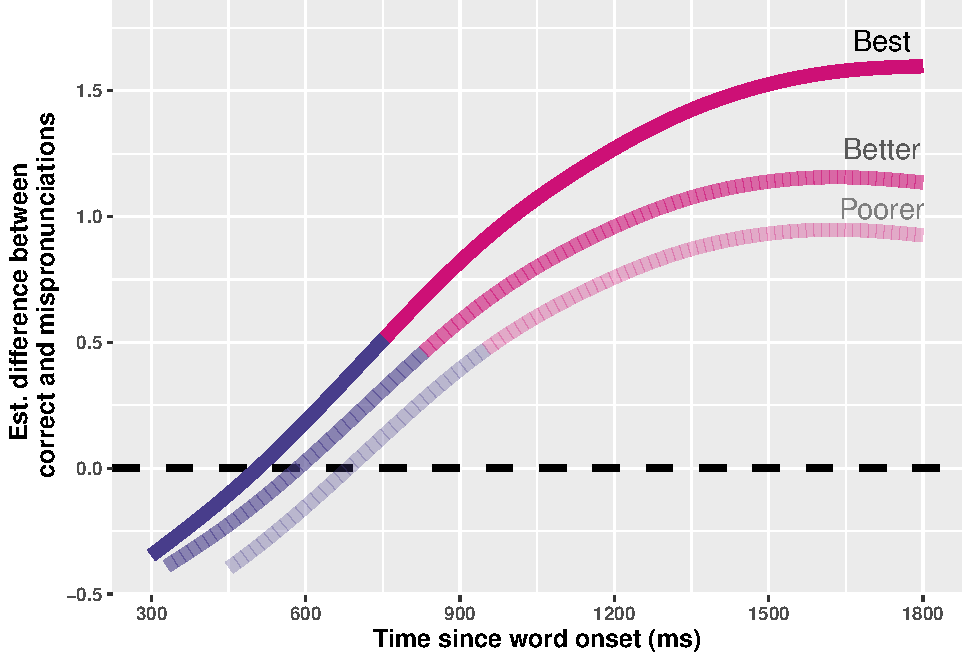
\includegraphics{2_modeling_files/figure-latex/CI-diff-plot-1.pdf}
\caption{\label{fig:CI-diff-plot}Difference smooths (GAMM predictions) between correct- and mis-pronunciations for children with CIs, by standardized articulation score. Pink smooths represent the point when correct- and mis-pronunciations smooths significantly differ (i.e., reliable effect of condition). Children were divided into tertiles by score with smooths representing the median score for children with poorer (median score=57), better (72), and best (96) articulation scores.}
\end{figure}

\begin{figure}
\centering
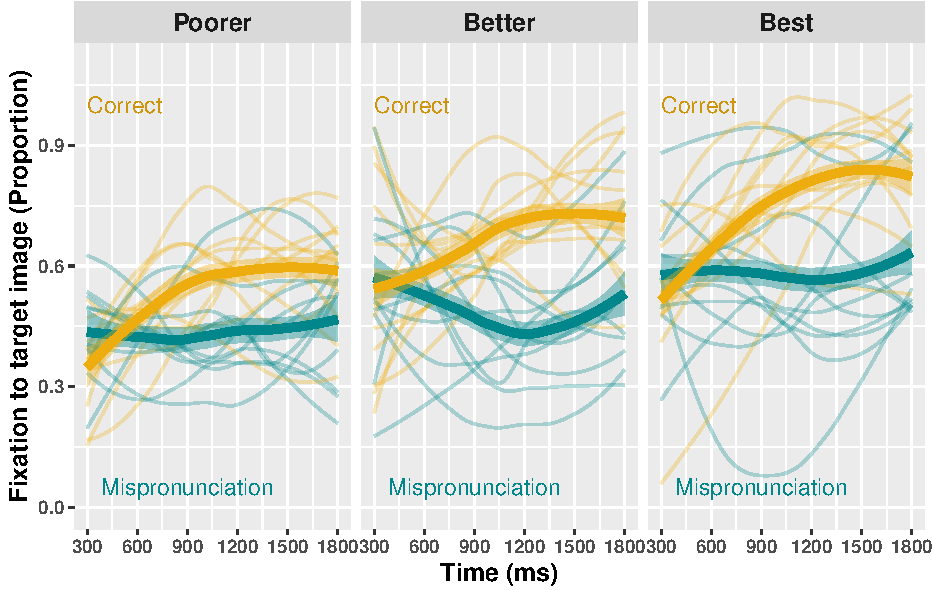
\includegraphics{2_modeling_files/figure-latex/CI-raw-plot-1.pdf}
\caption{\label{fig:CI-raw-plot}Raw response trajectories for proportion of looks to familiar object for children with CIs, by word condition and standardized articulation score. Children were divided into tertiles by score: poorer (median score=57), better (72), and best (96) articulation scores.}
\end{figure}

\hypertarget{appendices}{%
\section{Appendices}\label{appendices}}

\begin{table}[!h]

\caption{\label{tab:audiological-info}Audiological information from the N=25 unique children with cochlear implants studied.}
\centering
\begin{tabular}[t]{llrlrrlll}
\toprule
Participant & Matched to child with TH? & Chronological age & Age at hearing loss & Age at activation & Hearing age & Etiology & Device formation & Activation order\\
\midrule
300E & Y & 57 & 0 & 13 & 44 & Genetic & Bilateral & simultaneous\\
302E & Y & 37 & 0 & 13 & 24 & Unknown & Bilateral & R-L\\
303E & Y & 65 & 6 & 13 & 52 & Unknown & Bilateral & simultaneous\\
304E & Y & 48 & 0 & 12 & 36 & Genetic & Bilateral & R-L\\
305E & Y & 44 & 0 & 22 & 22 & Unknown & Bilateral & R-L\\
\addlinespace
306E & Y & 49 & 0 & 8 & 41 & Unknown & Bilateral & R-L\\
307E & Y & 44 & 0 & 15 & 29 & Genetic & Bilateral & R-L\\
309E & Y & 59 & 0.5 & 7 & 52 & Genetic & Bilateral & simultaneous\\
311E & Y & 62 & 9 & 13 & 49 & Unknown & Bilateral & L-R\\
314E & Y & 38 & 10 & 17 & 21 & Unknown & Bilateral & R-L\\
\addlinespace
608L & Y & 55 & 0.5 & 9 & 46 & Connexin 26 & Bilateral & simultaneous\\
665L & Y & 40 & 0 & 12 & 28 & Genetic & Bilateral & R-L\\
801E & Y & 39 & 1.5 & 15 & 24 & Unknown & Bilateral & simultaneous\\
804E & Y & 56 & 0 & 7 & 49 & Genetic & Bilateral & simultaneous\\
809E & Y & 64 & 6 & 8 & 56 & Meningitis & Bilateral & R-L\\
\addlinespace
301E & N & 53 & 0 & 45 & 8 & Unknown & Bilateral & R-L\\
308E & N & 37 & 0 & 13 & 24 & Genetic & Bilateral & simultaneous\\
310E & N & 52 & unknown & 23 & 29 & Genetic & Bilateral & simultaneous\\
312E & N & 57 & 0 & 24 & 33 & Genetic & Bilateral & R-L\\
679L & N & 58 & 0 & 29 & 29 & Genetic & Bimodal & n/a\\
\addlinespace
800E & N & 65 & 30 & 37 & 28 & Genetic & Bilateral & simultaneous\\
803E & N & 41 & 0 & 34 & 7 & Unknown & Bimodal & n/a\\
806E & N & 42 & 14 & 34 & 8 & Genetic & Unilateral & L\\
807E & N & 51 & 10 & 22 & 29 & Mondini malformation & Bimodal & n/a\\
808E & N & 37 & 0 & 6 & 31 & Genetic & Bilateral & simultaneous\\
\bottomrule
\end{tabular}
\end{table}

\hypertarget{supplementary-materials}{%
\section{Supplementary Materials}\label{supplementary-materials}}

\begin{verbatim}
## % latex table generated in R 4.0.2 by xtable 1.8-4 package
## % Tue May 17 12:24:02 2022
## \begin{table}[ht]
## \centering
## \begin{tabular}{lrrrr}
##    \hline
## A. parametric coefficients & Estimate & Std. Error & t-value & p-value \\ 
##   Intercept (Cochlear Implant: Mispronunciation) & 0.2560 & 0.1922 & 1.3325 & 0.1827 \\ 
##   Typical Hearing & -0.3070 & 0.1918 & -1.6007 & 0.1095 \\ 
##    \hline
## B. smooth terms & edf & Ref.df & F-value & p-value \\ 
##   s(Time) & 1.0826 & 1.5820 & 6.3116 & 0.0212 \\ 
##   s(Time,Cochlear Implant) & 1.0001 & 1.0002 & 0.5928 & 0.4414 \\ 
##   s(Time,Typical Hearing) & 1.0039 & 1.0072 & 5.5500 & 0.0182 \\ 
##   s(Time,Cochlear Implant Correct - Cochlear Implant Mispronunciation) & 6.0112 & 7.2081 & 8.2213 & $<$ 0.0001 \\ 
##   s(Time,Typical Hearing Difference - Cochlear Implant Difference) & 2.0002 & 2.0004 & 5.3745 & 0.0046 \\ 
##   s(Time,Child) & 52.1398 & 340.0000 & 0.4644 & $<$ 0.0001 \\ 
##   s(Time,Item) & 25.7681 & 106.0000 & 0.7128 & $<$ 0.0001 \\ 
##   s(Time,Observation) & 0.0014 & 26.0000 & 0.0003 & $<$ 0.0001 \\ 
##    \hline
## \end{tabular}
## \caption{Predicting the degree of mispronunciation sensitivity by hearing status.} 
## \label{tab.gam}
## \end{table}
\end{verbatim}

\begin{verbatim}
## % latex table generated in R 4.0.2 by xtable 1.8-4 package
## % Tue May 17 12:24:13 2022
## \begin{table}[ht]
## \centering
## \begin{tabular}{lrrrr}
##    \hline
## A. parametric coefficients & Estimate & Std. Error & t-value & p-value \\ 
##   Intercept (Mispronunciation) & 0.0835 & 0.1704 & 0.4900 & 0.6241 \\ 
##   Correct & 0.7110 & 0.1915 & 3.7131 & 0.0002 \\ 
##    \hline
## B. smooth terms & edf & Ref.df & F-value & p-value \\ 
##   s(Time) & 0.0006 & 9.0000 & 0.0001 & 0.0413 \\ 
##   s(Time,Correct) & 3.1503 & 9.0000 & 2.3435 & $<$ 0.0001 \\ 
##   s(Age) & 0.6289 & 9.0000 & 0.1893 & 0.0081 \\ 
##   te(Time,Age; Correct) & 3.1548 & 24.0000 & 0.3734 & 0.0049 \\ 
##   te(Time,Phonetic Accuracy; Correct) & 3.0315 & 24.0000 & 0.4423 & 0.0013 \\ 
##   s(Time,Child) & 48.6931 & 296.0000 & 0.2923 & $<$ 0.0001 \\ 
##   s(Time,Item) & 12.9259 & 106.0000 & 0.2786 & 0.0002 \\ 
##   s(Time,Observation) & 0.5166 & 26.0000 & 0.0299 & 0.0223 \\ 
##   s(Time,Child; Correct) & 0.0027 & 296.0000 & 0.0255 & $<$ 0.0001 \\ 
##    \hline
## \end{tabular}
## \caption{Predicting the degree of mispronunciation sensitivity by phonetic accuracy score.} 
## \label{tab.gam}
## \end{table}
\end{verbatim}

\end{document}
